%%%% CS 224N: Assignment #2 %%%%
%\documentclass[fleqn,10pt]{article}
%\usepackage{simplemargins}
%\setallmargins{1.0in}
\documentclass[10pt,reqno]{amsart}
\usepackage{amsmath}
\usepackage{amssymb}
\usepackage{amsthm}
\usepackage{bm}
\usepackage{enumitem}
\usepackage{graphicx}
\usepackage[paper=letterpaper,margin=0.6in]{geometry}
\usepackage[all]{xy}


%% Quick fix for wrapping text within a table column
\usepackage{array}
\newcolumntype{L}{>{\centering\arraybackslash}m{3cm}}


%% Define header
\begin{document}
\title{CS224n: Natural Language Processing with Deep Learning\\Assignment \#2}
\author{Anthony Ho}
\maketitle


%% Define shortcuts
\newcommand{\f}{\frac}
\newcommand{\pd}[1]{\frac{\partial}{\partial #1}}
\newcommand{\pdd}[2]{\frac{\partial #1}{\partial #2}}
\newcommand{\softmax}{\text{softmax}}


%% Set up numbering environment
\renewcommand{\labelenumi}{\arabic{enumi}.}
\begin{enumerate}[topsep=0pt,itemsep=3ex,partopsep=1ex,parsep=1ex]


%% Question 1
\item
  \begin{enumerate}[itemsep=2ex]
  %% Question 1(a)
  \item Please see the coding portion of the assignment.
  %% Question 1(b)
  \item Please see the coding portion of the assignment.
  %% Question 1(c)
  \item
    The purpose of the placeholder variables is to allocate storage for data/labels 
    before building the computation graph. The feed dictionaries allows us to inject 
    data/labels into the placeholders in a computation graph. 

    Please see the coding portion of the assignment for implementation. 
  %% Question 1(d)
  \item Please see the coding portion of the assignment.
  %% Question 1(e)
  \item 
    When the model's \texttt{train\_op} is called, 
    (1) it creates a gradient descent optimizer;
    (2) it calls \texttt{add\_loss\_op} to compute the cross entropy loss based on 
    the data, labels, and current values of the variables \texttt{W} and \texttt{b};
    (3) it computes the gradients w.r.t the loss via automatic differentiation;
    (4) and at the end it updates the values of the variables \texttt{W} and \texttt{b} in the direction
    of the gradient and in proportion to the learning rate as defined in \texttt{Config}.
    
    Please see the coding portion of the assignment for implementation. 
  \end{enumerate}


%% Question 2
\item
  \begin{enumerate}[itemsep=2ex]
  %% Question 2(a)
  \item The sequence of transitions are:
    \vspace{1mm}
    \begin{center}
      \begin{tabular}{l|l|l|l}
        stack & buffer & new dependency & transition \\
        \hline
        {[ROOT]} & [I, parsed, this, sentence, correctly] &  & Initial Configuration \\
        {[ROOT, I]} & [parsed, this, sentence, correctly] &  & \texttt{SHIFT} \\
        {[ROOT, I, parsed]} & [this, sentence, correctly] &  & \texttt{SHIFT} \\
        {[ROOT, parsed]} & [this, sentence, correctly] & parsed$\to$I & \texttt{LEFT-ARC} \\
        {[ROOT, parsed, this]} & [sentence, correctly] &  & \texttt{SHIFT} \\
        {[ROOT, parsed, this, sentence]} & [correctly] &  & \texttt{SHIFT} \\
        {[ROOT, parsed, sentence]} & [correctly] & sentence$\to$this  & \texttt{LEFT-ARC} \\
        {[ROOT, parsed]} & [correctly] & parsed$\to$sentence  & \texttt{RIGHT-ARC} \\
        {[ROOT, parsed, correctly]} & [] &  & \texttt{SHIFT} \\
        {[ROOT, parsed]} & [] & parsed$\to$correctly & \texttt{RIGHT-ARC} \\
        {[ROOT]} & [] & ROOT$\to$parsed & \texttt{RIGHT-ARC} \\
      \end{tabular}
    \end{center}
    \vspace{1mm}
  %% Question 2(b)
  \item A sentence containing $n$ words will be parsed in $2n$ steps,
    since each word must be first shifted from the buffer into the stack and
    then removed from the stack as a dependent of another item. 
  %% Question 2(c)
  \item Please see the coding portion of the assignment.
  %% Question 2(d)
  \item Please see the coding portion of the assignment.
  %% Question 2(e)
  \item Please see the coding portion of the assignment.
  %% Question 2(f)
  \item 
    For the following equation to be true:
    \begin{equation*}
      \mathbb{E}_{p_{drop}} [\bm{h}_{drop}]_i = h_i
    \end{equation*}
    $\gamma$ must fulfill the following criteria:
    \begin{align*}
      \mathbb{E}_{p_{drop}} [\bm{h}_{drop}]_i &= h_i \\
      \implies \gamma (1 - p_{drop}) h_i &= h_i \\
      \implies \gamma &= \f{1}{1 - p_{drop}} \\
    \end{align*}
  %% Question 2(g)
  \item 
    \begin{enumerate}[itemsep=2ex]
      \item By using $\bm{m}$ and a $\beta_1$ of 0.9, the new $\bm{\theta}$ would only 
        be updated slightly towards the new direction and would be largely the same 
        as the previous $\bm{\theta}$. It helps the 
        updates in $\bm{\theta}$ to maintain a relatively steady trajectory and prevents 
        the updates from ``diffusing around'' too much, and thus helps speeding up 
        reaching the local optimum. 
      \item Since Adam divides the updates by $\sqrt{\bm{v}}$, the model parameters that 
        have smaller magnitudes will get larger updates. This might help with combating 
        the ``saturated neurons'' problem by giving a ``boost'' to the updates of 
        the parameters that are ``saturated'' to get out of the ``plateaus''.
    \end{enumerate}
  %% Question 2(h)
  \item Please see the coding portion of the assignment for implementation.
    The best UAS achieved on the dev set is 88.66 
    and the UAS achieved on the test is 89.17. 
  \end{enumerate}


%% Question 3
\item
  \begin{enumerate}[itemsep=2ex]
  %% Question 3(a)
  \item
    \begin{enumerate}[itemsep=2ex]
      \item Let's denote $k$ as the index for the target word. Since $\bm{y}^{(t)}$ is a 
        one-hot vector:
        \begin{equation}
          \text{PP}^{(t)}\left(\bm{y}^{(t)}, \bm{\hat{y}}^{(t)}\right) 
          = \f{1}{\sum^{|V|}_{j=1} y^{(t)}_i \cdot \hat{y}^{(t)}_i}
          = \f{1}{\hat{y}^{(t)}_k} \label{3ai}
        \end{equation}
        and:
        \begin{equation}
          CE(\bm{y}^{(t)}, \bm{\hat{y}}^{(t)})
          = - \sum^{|V|}_{j=1} y^{(t)}_i \log \hat{y}^{(t)}_i
          = - \log \hat{y}^{(t)}_k \label{3aii}
        \end{equation}
        Therefore, combining equation (\ref{3ai}) and (\ref{3aii}):
        \begin{equation}
          CE(\bm{y}^{(t)}, \bm{\hat{y}}^{(t)})
          = - \log \hat{y}^{(t)}_k
          = - \log \f{1}{\text{PP}^{(t)}(\bm{y}^{(t)}, \bm{\hat{y}}^{(t)})}
          = \log \text{PP}^{(t)}(\bm{y}^{(t)}, \bm{\hat{y}}^{(t)}) \label{3aiii}
        \end{equation}
      \item
        We can rewrite the log of geometric mean perplexity using equation (\ref{3aiii}):
        \begin{align*}
          \log \left( \prod^T_{t=1} \text{PP}^{(t)}(\bm{y}^{(t)}, \bm{\hat{y}}^{(t)}) \right)^{1/T}
          &= \f{1}{T} \log \left( \prod^T_{t=1} \text{PP}^{(t)}(\bm{y}^{(t)}, \bm{\hat{y}}^{(t)}) \right) \\
          &= \f{1}{T} \sum^T_{t=1} \log \text{PP}^{(t)}(\bm{y}^{(t)}, \bm{\hat{y}}^{(t)}) \\
          &= \f{1}{T} \sum^T_{t=1} CE(\bm{y}^{(t)}, \bm{\hat{y}}^{(t)})
        \end{align*}
        Since $\left( \prod^T_{t=1} \text{PP}^{(t)}(\bm{y}^{(t)}, \bm{\hat{y}}^{(t)}) \right)^{1/T}$ is 
        a positive function, minimizing 
        $\log \left( \prod^T_{t=1} \text{PP}^{(t)}(\bm{y}^{(t)}, \bm{\hat{y}}^{(t)}) \right)^{1/T}$
        is equivalent to minimizing 
        $\left( \prod^T_{t=1} \text{PP}^{(t)}(\bm{y}^{(t)}, \bm{\hat{y}}^{(t)}) \right)^{1/T}$ itself. 
        Therefore, minimizing the geometric mean perplexity 
        $\left( \prod^T_{t=1} \text{PP}^{(t)}(\bm{y}^{(t)}, \bm{\hat{y}}^{(t)}) \right)^{1/T}$
        is equivalent to minimizing the arithmetic mean cross-entropy loss 
        $\f{1}{T} \sum^T_{t=1} CE(\bm{y}^{(t)}, \bm{\hat{y}}^{(t)})$. 
      \item
        If $\bar{P}(\bm{x}^{(t+1)}_\text{pred} = \bm{x}^{(t+1)} | \bm{x}^{(t)}, \dots, \bm{x}^{(1)}) = 1/|V|$,
        it means $\text{PP}^{(t)}(\bm{y}^{(t)}, \bm{\hat{y}}^{(t)}) = 1/(1/|V|) = |V|$. 
        When $|V| = 10000$, the corresponding cross-entropy loss is $\log(10000) = 9.21$.
    \end{enumerate}
  %% Question 3(b)
  \item
    Let's denote:
    \begin{align*}
      \bm{z}^{(t)} &= \bm{W}_h \bm{h}^{(t-1)} + \bm{W}_e \bm{e}^{(t)} + \bm{b}_1 \in \mathbb{R}^{D_h\times1} \\
      \bm{\theta}^{(t)} &= \bm{U} \bm{h}^{(t)} + \bm{b}_2 \in \mathbb{R}^{|V|\times1} 
    \end{align*}

    We can define and compute the values of the following error terms:
    \begin{align*}
      \bm{\sigma}^{(t)}_1 &= \pdd{J^{(t)}}{\bm{\theta}^{(t)}}
      = \pdd{CE(\bm{y}^{(t)}, \bm{\hat{y}}^{(t)})}{\bm{\theta}^{(t)}}
      = \bm{\hat{y}}^{(t)} - \bm{y}^{(t)} 
      \in \mathbb{R}^{|V|\times1} \\
      \bm{\sigma}^{(t)}_2 &= \pdd{J^{(t)}}{\bm{z}^{(t)}}
      = \bm{\sigma}^{(t)}_1 \pdd{\bm{\theta}^{(t)}}{\bm{h}^{(t)}} \pdd{\bm{h}^{(t)}}{\bm{z}^{(t)}}
      = \bm{U}^\top \left(\bm{\hat{y}}^{(t)} - \bm{y}^{(t)} \right) \circ \bm{h}^{(t)} \circ (1 - \bm{h}^{(t)})
      \in \mathbb{R}^{D_h\times1}
    \end{align*}
    
    Therefore, 
    \begin{align*}
      \pdd{J^{(t)}}{\bm{U}}
      &= \pdd{J^{(t)}}{\bm{\theta}^{(t)}} \pdd{\bm{\theta}^{(t)}}{\bm{U}}
      = \bm{\sigma}^{(t)}_1 \left(\bm{h}^{(t)}\right)^\top
      \in \mathbb{R}^{|V|\times D_h} \\
      \pdd{J^{(t)}}{\bm{e}^{(t)}}
      &= \pdd{J^{(t)}}{\bm{z}^{(t)}} \pdd{\bm{z}^{(t)}}{\bm{e}^{(t)}} 
      = \bm{W}_e^\top \bm{\sigma}^{(t)}_2 
      \in \mathbb{R}^{d\times 1} \\
      \left. \pdd{J^{(t)}}{\bm{W}_e} \right\rvert_{(t)}
      &= \pdd{J^{(t)}}{\bm{z}^{(t)}} \left. \pdd{\bm{z}^{(t)}}{\bm{W}_e} \right\rvert_{(t)}
      = \bm{\sigma}^{(t)}_2 \left(\bm{e}^{(t)}\right)^\top
      \in \mathbb{R}^{D_h \times d} \\
      \left. \pdd{J^{(t)}}{\bm{W}_h} \right\rvert_{(t)}
      &= \pdd{J^{(t)}}{\bm{z}^{(t)}} \left. \pdd{\bm{z}^{(t)}}{\bm{W}_h} \right\rvert_{(t)}
      = \bm{\sigma}^{(t)}_2 \left(\bm{h}^{(t-1)}\right)^\top
      \in \mathbb{R}^{D_h \times D_h} \\
      \pdd{J^{(t)}}{\bm{h}^{(t-1)}}
      &= \pdd{J^{(t)}}{\bm{z}^{(t)}}  \pdd{\bm{z}^{(t)}}{\bm{h}^{(t-1)}} 
      = \bm{W}_h^\top \bm{\sigma}^{(t)}_2 
      \in \mathbb{R}^{D_h\times 1} 
    \end{align*}
  %% Question 3(c)
  \item The ``unrolled''network for 3 timesteps is shown in figure \ref{fig1}.
    \begin{figure}[h]
      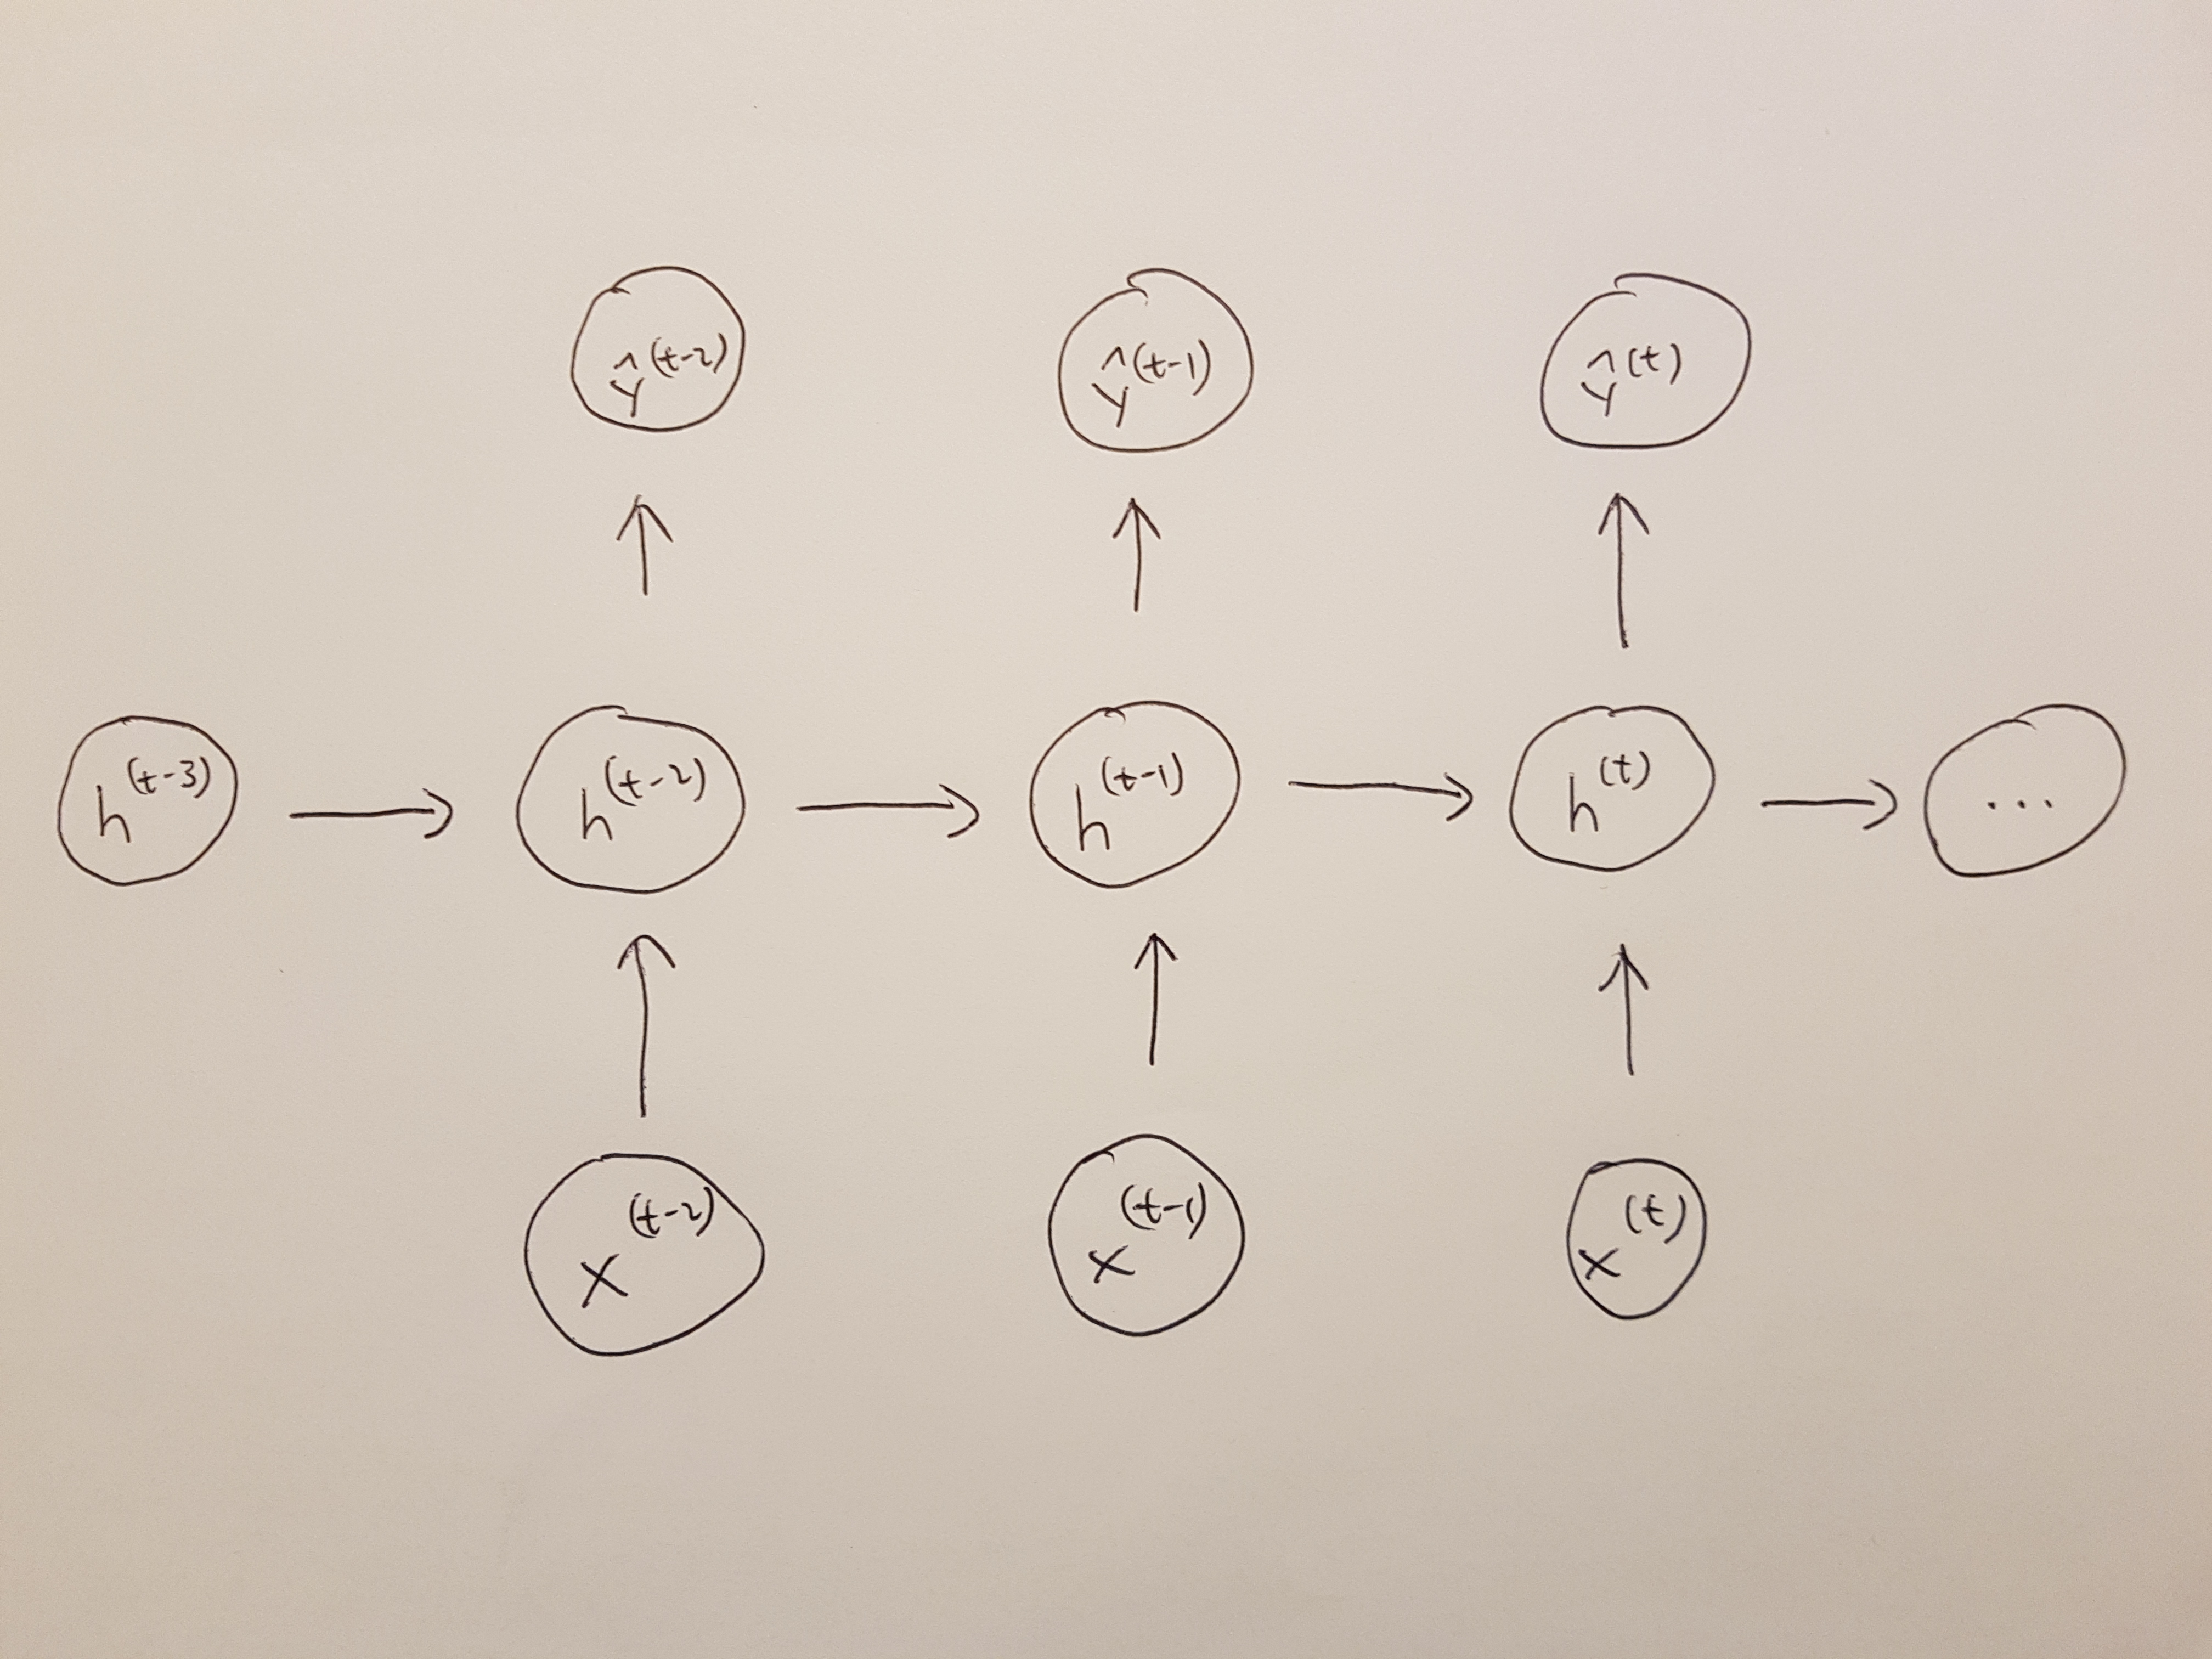
\includegraphics[width=0.6\textwidth]{q3c.jpg}
      \caption{The ``unrolled''network for 3 timesteps.}
      \label{fig1}
    \end{figure}

    Let's compute the gradient of $J^{(t)}$ w.r.t. $\bm{z}^{(t-1)}$:
    \begin{equation*}
      \pdd{J^{(t)}}{\bm{z}^{(t-1)}} 
      = \pdd{J^{(t)}}{\bm{h}^{(t-1)}} \pdd{\bm{h}^{(t-1)}}{\bm{z}^{(t-1)}}
      = \bm{\gamma}^{(t-1)} \circ \bm{h}^{(t-1)} \circ (1 - \bm{h}^{(t-1)}) 
      \in \mathbb{R}^{D_h\times 1} 
    \end{equation*}

    Therefore,
    \begin{align*}
      \pdd{J^{(t)}}{\bm{e}^{(t-1)}}
      &= \pdd{J^{(t)}}{\bm{z}^{(t-1)}} \pdd{\bm{z}^{(t-1)}}{\bm{e}^{(t-1)}} 
      = \bm{W}_e^\top \left( \bm{\gamma}^{(t-1)} \circ \bm{h}^{(t-1)} \circ (1 - \bm{h}^{(t-1)}) \right)
      \in \mathbb{R}^{d\times 1} \\
      \left. \pdd{J^{(t)}}{\bm{W}_e} \right\rvert_{(t-1)}
      &= \pdd{J^{(t)}}{\bm{z}^{(t-1)}} \left. \pdd{\bm{z}^{(t-1)}}{\bm{W}_e} \right\rvert_{(t-1)}
      = \left( \bm{\gamma}^{(t-1)} \circ \bm{h}^{(t-1)} \circ (1 - \bm{h}^{(t-1)}) \right) \left(\bm{e}^{(t-1)}\right)^\top
      \in \mathbb{R}^{D_h \times d} \\
      \left. \pdd{J^{(t)}}{\bm{W}_h} \right\rvert_{(t-1)}
      &= \pdd{J^{(t)}}{\bm{z}^{(t-1)}} \left. \pdd{\bm{z}^{(t-1)}}{\bm{W}_h} \right\rvert_{(t-1)}
      = \left( \bm{\gamma}^{(t-1)} \circ \bm{h}^{(t-1)} \circ (1 - \bm{h}^{(t-1)}) \right) \left(\bm{h}^{(t-2)}\right)^\top
      \in \mathbb{R}^{D_h \times D_h} 
    \end{align*}
  %% Question 3(d)
  \item    
  %% Question 3(e)
  \item 
  %% Question 3(f)
  \item 
  \end{enumerate}


\end{enumerate}
\end{document}
